\subsection{Excercise TestCarRentalCLI}
\label{sec:exercise_test_car_rental_cli}

\subsubsection*{Derive Test Cases}
For the sake of simplicity, we asume that a correct car called \texttt{correctCar} and customer called \texttt{correctCustomer} are provided.
In the cases where the date is correct we assume the date \texttt{startDate} and \texttt{endDate} represent correct dates.
In our case we assume the startDate to be the 01.01.2000 and the endDate to be the 02.02.2000.

First we define positive and negative test cases for the \texttt{NewRental} function.
\begin{lstlisting}[
style=kit-cm,
language=Golang,
caption={Test Cases for the Rental Context},
label={lstlisting:rental_test_cases},
]
// Constraint 1: self.ID -> notEmpty()
NewRental("", startDate, endDate, correctCar, correctCustomer) // negative test case
NewRental("Rental1", startDate, endDate, correctCar, correctCustomer) // positive test case

// Constraint 2: self.startDate -> notEmty()
NewRental("Rental2", date{}, endDate, correctCar, correctCustomer) // negative test case
NewRental("Rental2", startDate, endDate, correctCar, correctCustomer) // positive test case

// Constraint 3: self.endDate -> notEmty()
NewRental("Rental3", startDate, date{}, correctCar, correctCustomer) // negative test case
NewRental("Rental3", startDate, endDate, correctCar, correctCustomer) // positive test case

// Constraint 4: self.startDate < self.endDate
NewRental("Rental4", endDate, startDate, correctCar, correctCustomer) // negative test case
NewRental("Rental4", startDate, endDate, correctCar, correctCustomer) // positive test case

// Constraint 5: self.car -> notEmpty()
NewRental("Rental5", startDate, endDate, car{}, correctCustomer) // negative test case
NewRental("Rental5", startDate, endDate, correctCar, correctCustomer) // positive test case

// Constraint 6: self.customer -> notEmpty()
NewRental("Rental6", startDate, endDate, correctCar, customer{}) // negative test case
NewRental("Rental6", startDate, endDate, correctCar, correctCustomer) // positive test case
\end{lstlisting}
  
Now, we define positive and negative test cases for the \texttt{rentACar\(\)} function.
This function takes the rentalID, start and endDate, the car, and the customer as arguments.
If the function is executed correctly it will return the new rental.
We specified in the beginning of the section, startDate, endDate, correctCar, and correctCustomer represent correct parameters.

\begin{lstlisting}[
style=kit-cm,
language=Golang,
caption={Test Cases for the Customer Context},
label={lstlisting:customer_test_cases},
]
// Constraint 1: pre: self.rentalID -> not exists
rentACar("Rental1", startDate, endDate, correctCar, correctCustomer)
rentACar("Rental1", startDate, endDate, correctCar, correctCustomer) // negative test case due to function executing twice
rentACar("Rental2", startDate, endDate, correctCar, correctCustomer) // positive test case

// Constraint 2: and Rental.allInstances() -> 
//  forAll(r: Rental | r.car = self.car implies(self.endDate < r.endDate or r.Endate > self.startDate))
rentACar("Rental3", startDate, endDate, correctCar, correctCustomer)
rentACar("Rental4", startDate', endDate, correctCar, correctCustomer') // negative test case due to overlapping dates for the same car
rentACar("Rental5", startDate', endDate', correctCar, correctCustomer') // positive test case 

// Constraint 3: post: self.rentals -> includes(rental)
rentACar("Rental6", startDate, endDate, correctCar, correctCustomer) // positive test case
rentACar("Rental7", date{}, endDate, correctCar, correctCustomer) // negative test case => due to constraint 2, the element will not be created and therefore will not appear in the list

\end{lstlisting}

\subsubsection*{Analyze Test Structure}
% Structure description of the test file and mock-repository
The MockCarRepository acts similar to the actual CarRepository.
It implements the CarRentalRepositoryInterface and provides the according functions.
Furthermore, it also implements the lists of the models \texttt{Rental}, \texttt{Car}, and \texttt{Customer}.
However, there is no constructor and no manipulation of yaml files.
All data-manipulations are done in the memory of the mock-repository.
Therefore the mock-repository only imports the used models.

The test file \texttt{RentACarOperation\_test.go} implements the tests for the \texttt{RentACar} function.
It creates the testint environment by implementing the constructor of the mock-repository, populating it with test data.
After the setup the executable tests are implemented.

% Structure description of the test function TestCarRentalOperations_RentACar
The implementation of the tests happens in the \texttt{TestCarRentalOperations\_RentACar} function.
The \texttt{fields} struct defines the repository used in each test and therefore the test environment.
After that, the \texttt{args} struct defines the arguments needed for the \texttt{RentACar} function.
Now, the test cases are implemented containing the following values:
\begin{itemize}
      \item fields: The repository used in the test as specified above
      \item name: The name of the test
      \item args: The arguments for the \texttt{RentACar} function as specified above
      \item want: The expected return value of the \texttt{RentACar} function, in this case a String 
      \item wantErr: True, if an error is expected, false otherwise. 
            This allows the implementation of negative test cases without the tests failing.
\end{itemize}

% Differences between the mock and the normal repository
The following differences occur between the mock and the normal repository:
\begin{itemize}
      \item The mock repository does not implement a constructor
      \item The mock repository does not manipulate any yaml files, everything is done in the mock repository's lists.
      \item The mock repository only imports the models used in the tests.
      \item The mock repository is only used for testing while the normal repository is used in the application.
      \item The mock repository is located in the same package as the test file (operations), while the normal repository is located in the infrastructure package.
\end{itemize}

However, there are still some similarities:
\begin{itemize}
      \item Both repositories implement the CarRentalRepositoryInterface and therefore provide the same functions.
      \item The provided functionalities are somewhat similar besides the differences mentioned above.
      \item Both repositories are adressed via an operations object representing the repository
\end{itemize}

% Why is a mocked repository required?
Now, why is mocked repository required?
First of all, the mock repository is required to test the functionality of the \texttt{RentACar} function.
This could also be done with the normal repository, however, this would require the manipulation of the yaml files, which arises the following problems:
\begin{itemize}
      \item Test data and actual application data are mixed up
      \item The test data is not reset after the test, which could lead to problems in the next test
      \item The test data needs no be cleaned up after the test, which is not necessary with the mock repository
      \item By creating a certain testing environment, the testing data can manipulated to test the wanted scenarios
\end{itemize}

Further benefits and the actual usage and implementation of both the normal and the mock repository are further explained in \autoref{sec:go_repositories}.
As shown all tests pass besides the first test.
This is due to the given testing envorionment.
The rental is already created therefore an error will occur and the test fails.

\subsubsection*{Add Test Data}
%//TODO Prozess und Code vom Hinzufügen der Testdaten beschreiben

\subsubsection*{Implement Test Cases}
%//TODO Prozess und Code vom Hinzufügen der Testfälle beschreiben

\subsection*{Run Tests}
%//TODO Prozess und Ergebnisse weiter ausführen (wie wird der Code ausgeführt)
Test testing results are shown in \autoref{fig:carRentalCLI_testingConsoleOutput} and \autoref{fig:carRentalCLI_testingGraphicalOutput}.

The negative test-cases do not fail due to its construction.
By setting the \texttt{wantErr} value to true, the test will not fail if an error occurs.
This allows the implementation of negative test cases without the tests failing, which is the desired behaviour.

\begin{figure}
      \centering
      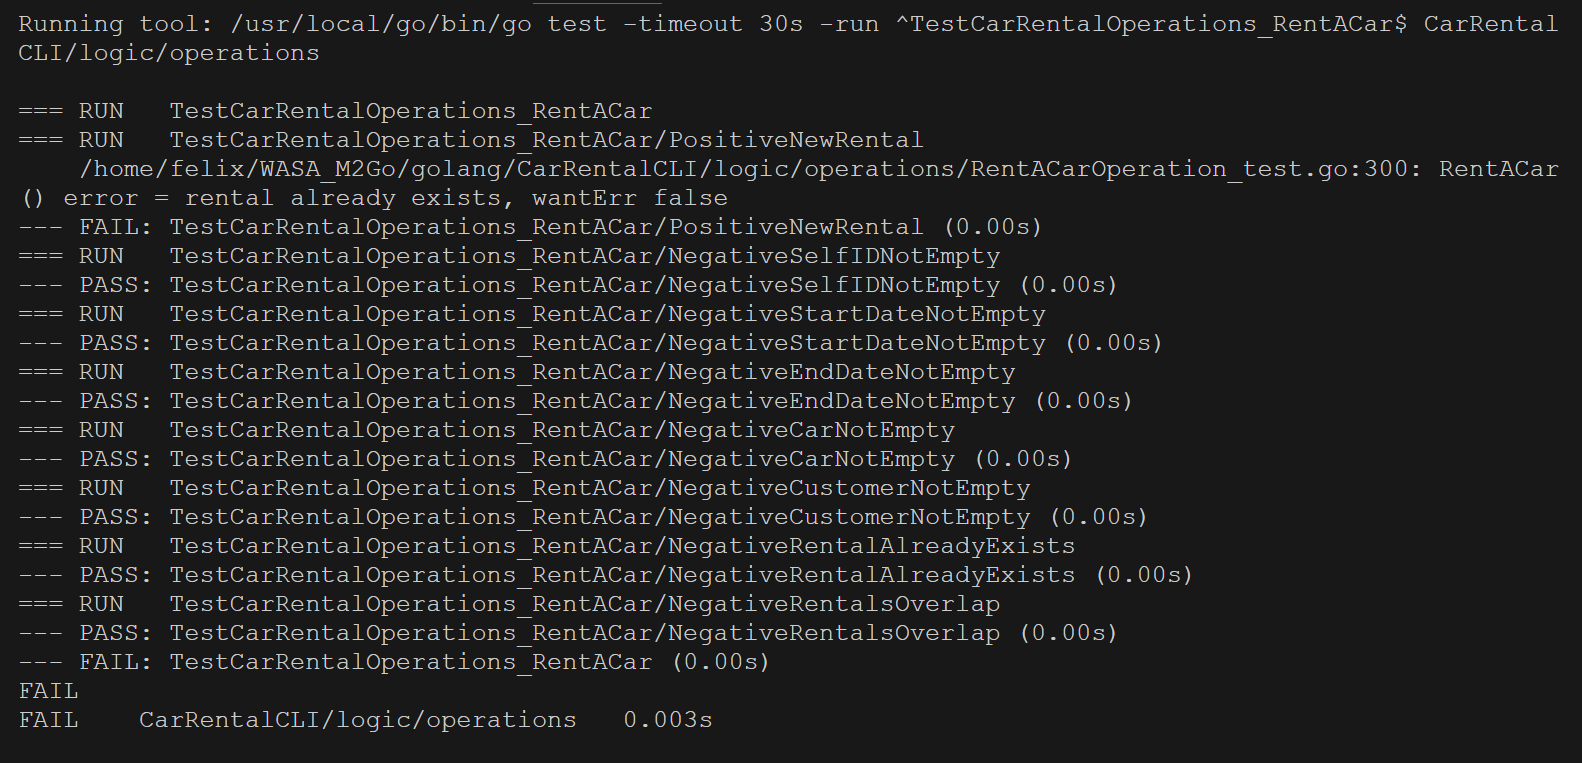
\includegraphics[width=0.8\textwidth]{figures/goLang/carRental/carRentalCLI/carRentalCLI_testingConsoleOutput.png}
      \caption{Console Output of the RentACar Tests}
      \label{fig:carRentalCLI_testingConsoleOutput}
\end{figure}
\begin{figure}
      \centering
      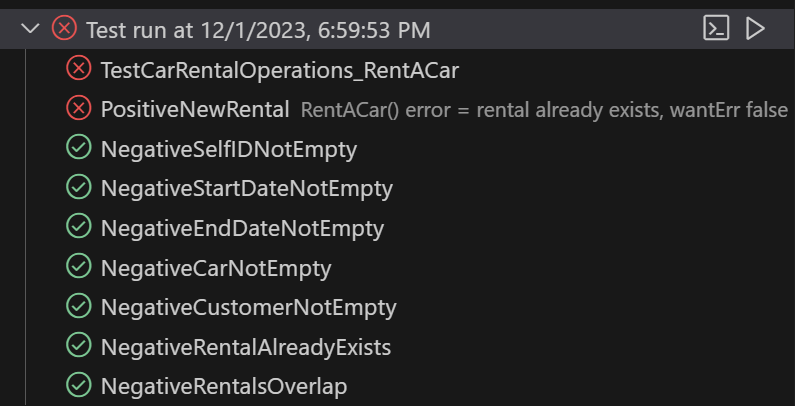
\includegraphics[width=0.8\textwidth]{figures/goLang/carRental/carRentalCLI/carRentalCLI_testingGraphicalOutput.png}
      \caption{Graphical Output of the RentACar Tests}
      \label{fig:carRentalCLI_testingGraphicalOutput}
\end{figure}



